
\chapter[Related Works]{State of the art}
\graphicspath{ {images/stateOfArt} }



\section{Software visualization}


\begin{wrapfigure}{r}{0.3\textwidth}

  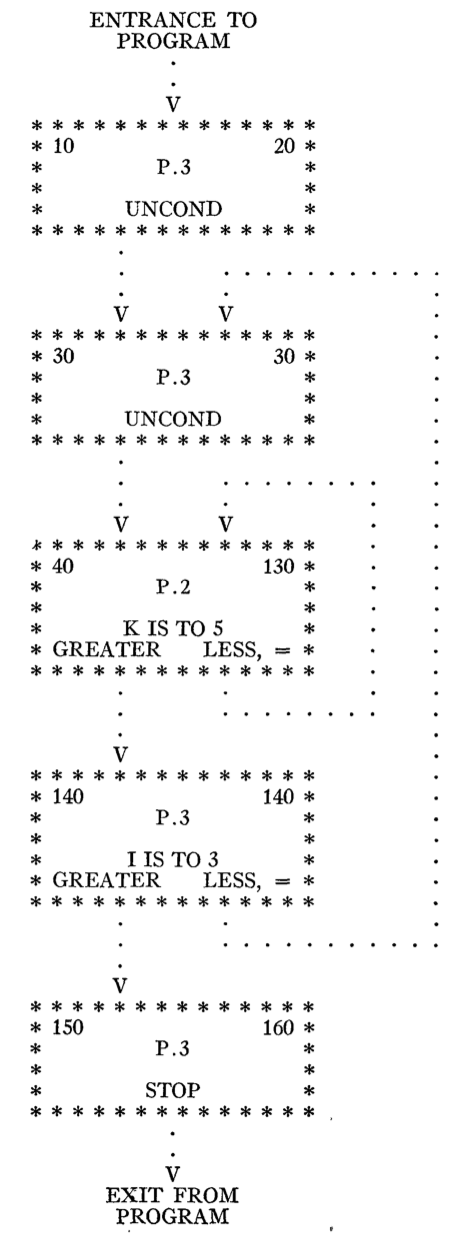
\includegraphics[width=0.9\linewidth]{Haibt1959_Flowchart.png} 
  \caption{Flowchart presented by Haibt in 1959}
  \label{fig:Haibt1959_Flowchart}

\end{wrapfigure}

Essential parts of software lifecycles are software maintenance and software evolution. 
Both activities require the comprehension of the system by the developer. 
Mayrhauser \cite{VonMayrhauser1995} defined program comprehension as a process that uses knowledge to acquire new knowledge. 
Generally, programmers possess two types of knowledge: general knowledge and software-specific knowledge, which represent their level of understanding of that software. 
Software comprehension aims to increase this specific knowledge of the system, and, to do that, it can leverage some software visualization techniques. 
Software visualization supports the understanding of software systems because it enables the visualization of the system's information (architecture, source code, behavior) with a 2D or 3D representation. 
Stasko et al.\cite{Stasko2008} conducted a study in 1998 that shows how visualization arguments human memory since it works as external cognitive aid and thus, improves thinking and analysis capabilities. \\

\subsection*{History of software visualization}



The earliest form of software visualization found in the literature was in the form of 2D diagrams. 
Haibt \cite{Haibt1959} in 1959, was one of the first to use them to visualize software systems. 
He provided a graphical outline of a program and its behavior with flowcharts. As shown in Figure \ref{fig:Haibt1959_Flowchart}, they 
were 2D diagrams that described the execution of a program. He wrapped each statement in a box, representing the control flow with arrows.
Ten years later, the effectiveness of flowcharts was confirmed by Knuth \cite{Knuth1963}. 
Unfortunately, at that time, most of the programs were affected by a lack of readability since they were not well documented. 
So, it introduced a tool to automatically generate visualizations from the software documentation. 
Nassi and Schneiderman\cite{Nassi1973}, in 1973, introduced the Nassi–Shneiderman diagram (NSD), able to represent the structure of a program. 
The diagram was divided into multiple sub-block, each with a given semantic based on its shape and position. 


The 80s registered two main directions of software visualization. The first was the source code presentation.
Hueras \cite{Hueras1977}, and Waters \cite{Waters1983} developed two techniques to format the source code with a prettyprinter. 
The second direction was the program behavior, used mainly for educational purposes. One of the most prominent visualization systems of that period was Balsa-II \cite{Brown1988}.
Around the end of the 80s, Müller et al. \cite{Mueller1988} released Rigi, a tool able to visualize large programs.
It exploited graph model, argumented with an abstraction mechanisms, to represent systems components and their relationships. 

\begin{figure}[H]
  \minipage{0.33\textwidth}
    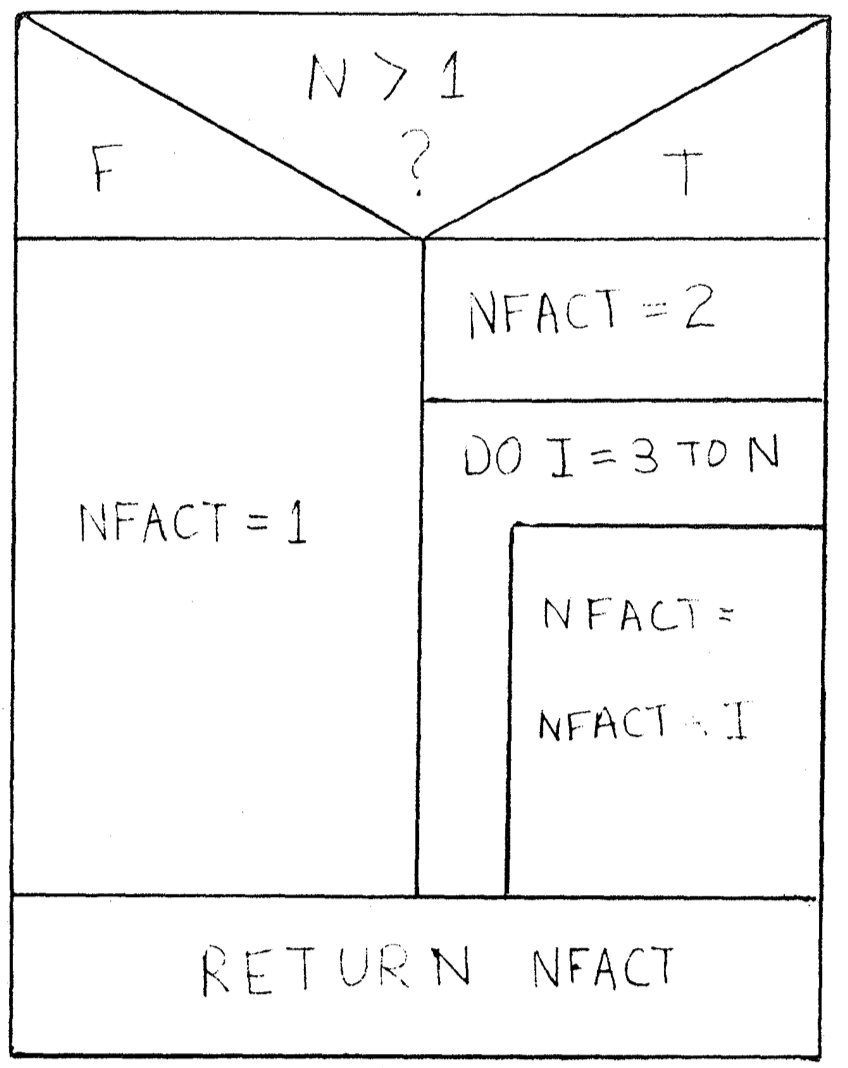
\includegraphics[width=0.8\linewidth]{Nassi1973_NSD.png}
    \label{fig:Nassi1973_NSD}
    \caption{NSD of the factorial function.}
  \endminipage\hfill
  \minipage{0.33\textwidth}
    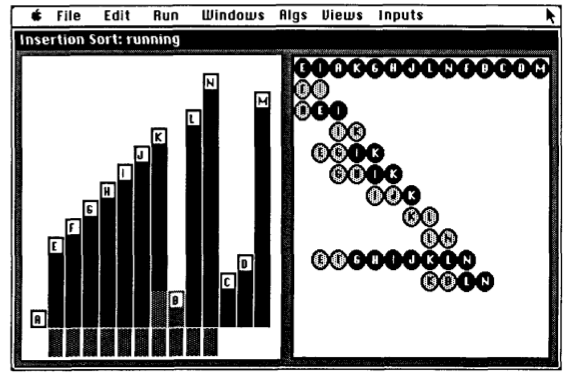
\includegraphics[width=\linewidth]{Brown1988_BalsaII.png}
    \caption{Balsa-II}
  \endminipage\hfill
  \minipage{0.33\textwidth}
  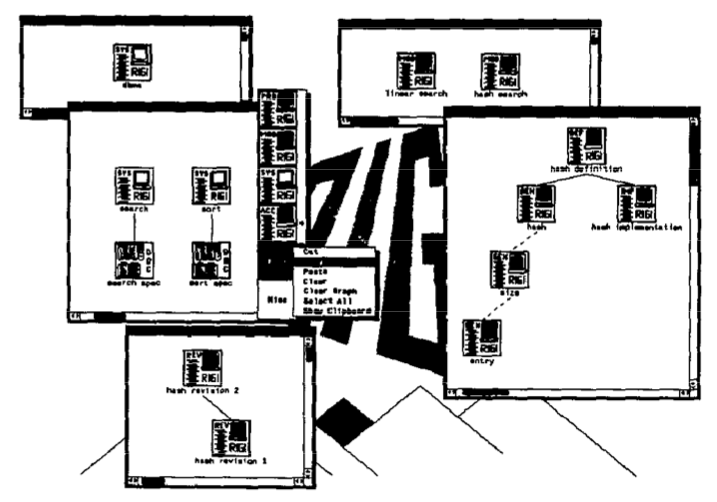
\includegraphics[width=\linewidth]{Mueller1988_Rigi.png}
  \caption{Rigi}
\endminipage\hfill
  \end{figure}


  % The growing number of object-oriented programming languages emerging in the mainstream raised 
  % the interest in understanding not only the structure, but also the behavior of systems written according to this paradigm. 
  % Kleyn et al. proposed GraphTrace [KG88], a tool using concurrently animated views to visualize dynamic information,
  % Myers’s taxonomy of program visualization systems
  % Price et al. proposed a more detailed taxonomy


The 1990s recorded more interest in the field of software visualization. 
In 1992 Erik et al \cite{Eick1992} introduced a new technique to visualize line oriented statistics. 
It was enboded in Seesoft, a software visualization system that allowed to analyze and visualize up to 50,000 lines of code simultaneously. 
On their visualization, each line was mapped to a thin row. Each row was associated with a color that described a statistic of interest.
One year later, De pauw et al. \cite{DePauw1993} introduced Jinsight, a tool able to provide animated views of the behavior of object-oriented systems. 

\begin{figure}[H]
  \minipage{0.5\textwidth}
    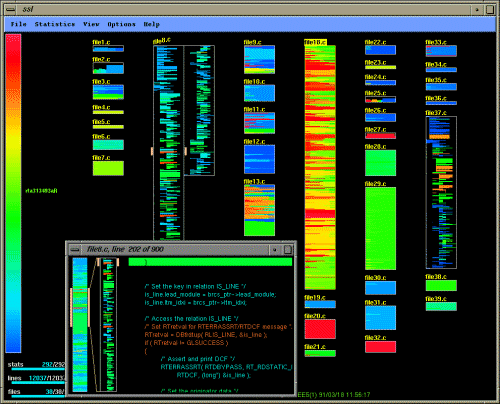
\includegraphics[width=0.8\linewidth]{Eick1992_Seesoft.png}
    \caption{Seesoft}
  \endminipage\hfill
  \minipage{0.5\textwidth}
    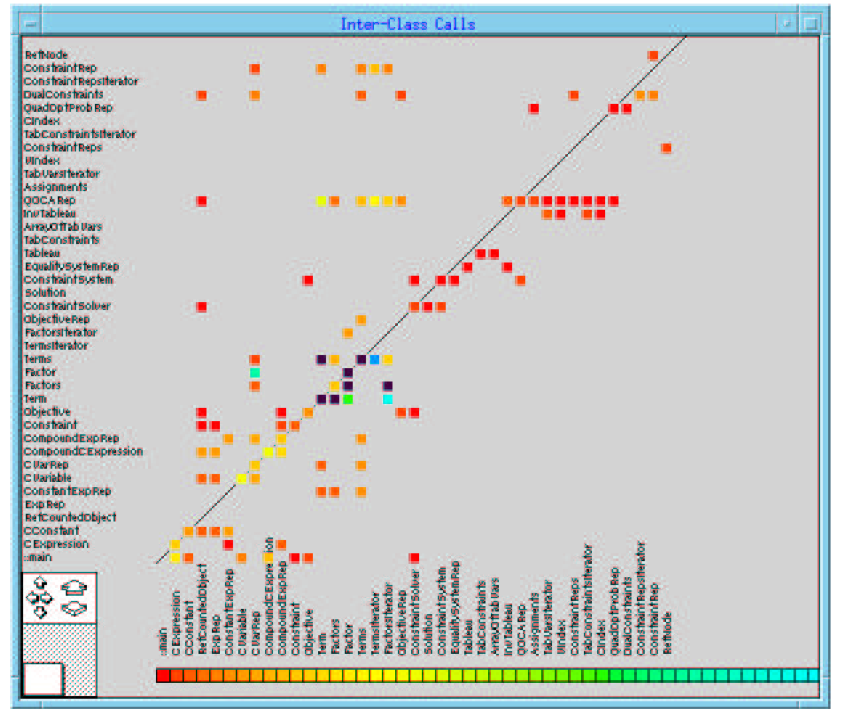
\includegraphics[width=0.8\linewidth]{DePauw1993_Jinsight.png}
    \caption{Jinsight}
  \endminipage\hfill
\end{figure}

% he first contributors to software evolution visualization were Holt and Pak in 1996, who used their tool called GASE [HP96]
% 		GASE: visualizing software evolution-in-the-large 

That period was favorable also for experimenting novel research directions for visualization, 
such as 3D visualization and Virtal Reality. 
% In 1995, Reiss presented a configurable engine for building 3D visualization of programs called PLUM
In 1998, Chuah and Erick \cite{Chuah1998} proposed three different techniques to visualize project data. 
They exploited the concept of glyphs, a graphical object that represents data through visual parameters. 
The first technique was the Timewhell glyph, used to visualize time-oriented information (number of lines of code, number of errors, number of added lines). 
The second technique was the 3D wheel glyph; it encoded the same attributes of the time wheel, and additionally, it used the height to encode time. 
Infobug glyph was the last technique, where each glyph was composed of four parts, each representing essential data of the system (time, code size, number of lines of code added/deleted/modified). \newline

\begin{figure}[H]
\minipage{0.32\textwidth}
  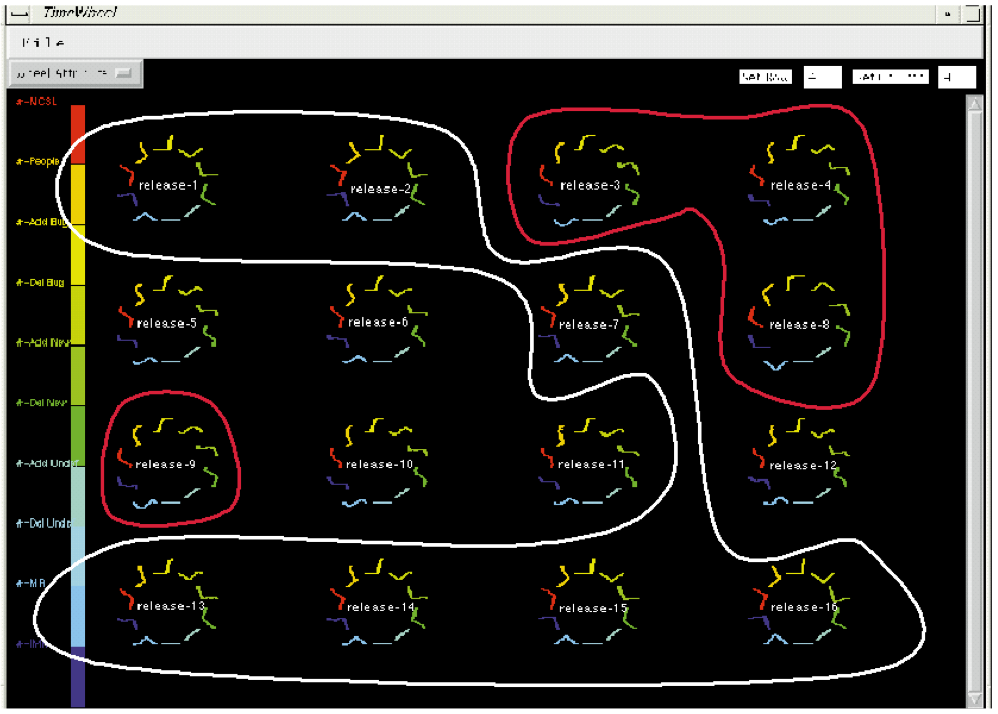
\includegraphics[width=\linewidth]{Chuan1.png}
  \caption{Timewhell}
\endminipage\hfill
\minipage{0.32\textwidth}
  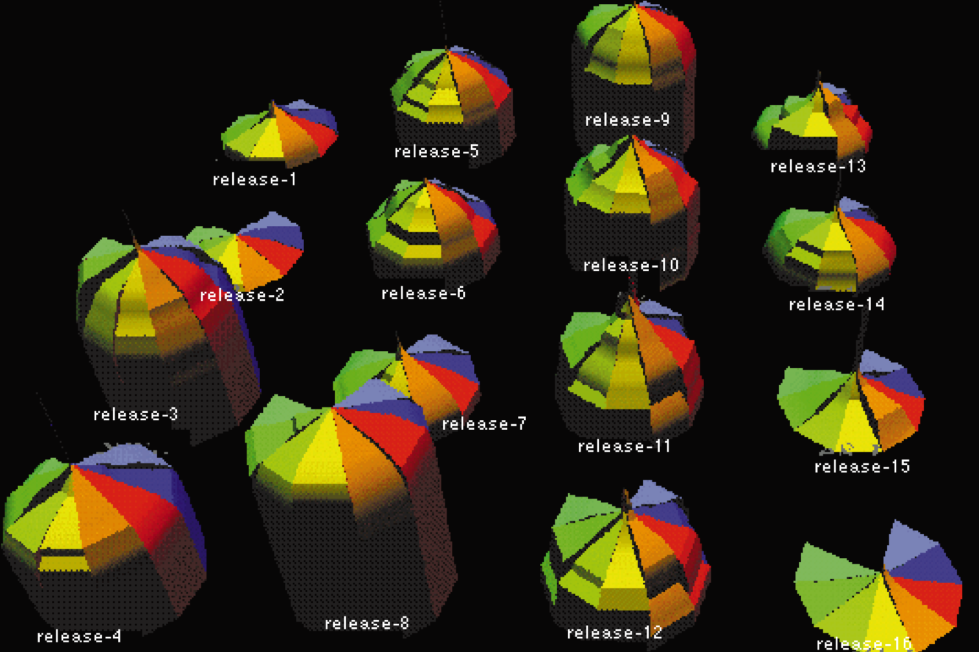
\includegraphics[width=\linewidth]{Chuan2.png}
  \caption{3D wheel}
\endminipage\hfill
\minipage{0.32\textwidth}%
  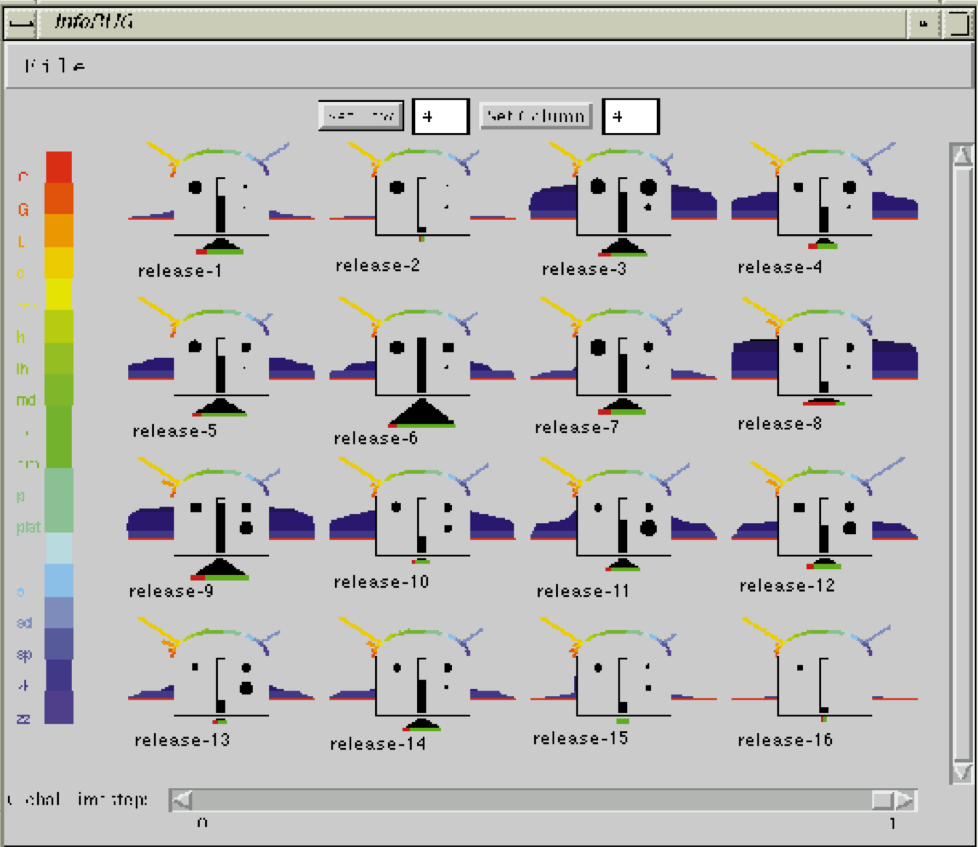
\includegraphics[width=\linewidth]{Chuan3.png}
  \caption{Infobug}
\endminipage
\end{figure}

In the same year, Young and Munro \cite{Young1998} explored representations of software for program comprehension in VR. 
Finally in 1999, Jacobson et al. \cite{Jacobson1999} introduced what we now know as de facto the standard language to visualize the design on a system: UML. 


% Edward Tufte has influenced the entire field of information visualization, including software visualization.
% 	[Tuf90] Edward Tufte. Envisioning Information. Graphics Press, 1990.
% 	[Tuf97] Edward Tufte. Visual Explanations. Graphics Press, 1997.
% 	[Tuf01] Edward Tufte. The Visual Display of Quantitative Information. Graphics Press, 2nd edition, 2001.

\subsection{Software evolution visualization}
Before the beginning of the 21st century, visualize the evolution of a system was an unfeasible task due to the lack of data. 
However, tanks to the spread of version control systems and of the open-souce movement, these information became publicy accessible.
As a result, may researchers focused their work on software evolution visualization.

In 2001 Lanza \cite{Lanza2001} introduced the concept of the Evolution Matrix. It was a way to visualize the evolution of software without dealing with a large amount of complex data. 
Furthermore, that approach was agnostic to any particular programming language. The Evolution Matrix aimed to display the evolution of classes in object-oriented software systems. 
Each column represented a version of the software, and each row represented a different version of the same class. The cells were filled with boxes whose size depended on two different metrics. 
Thanks to this approach, he was able to infer some evolution information by just looking at the shape of the matrix

\begin{figure}[H]
\minipage{0.49\textwidth}
  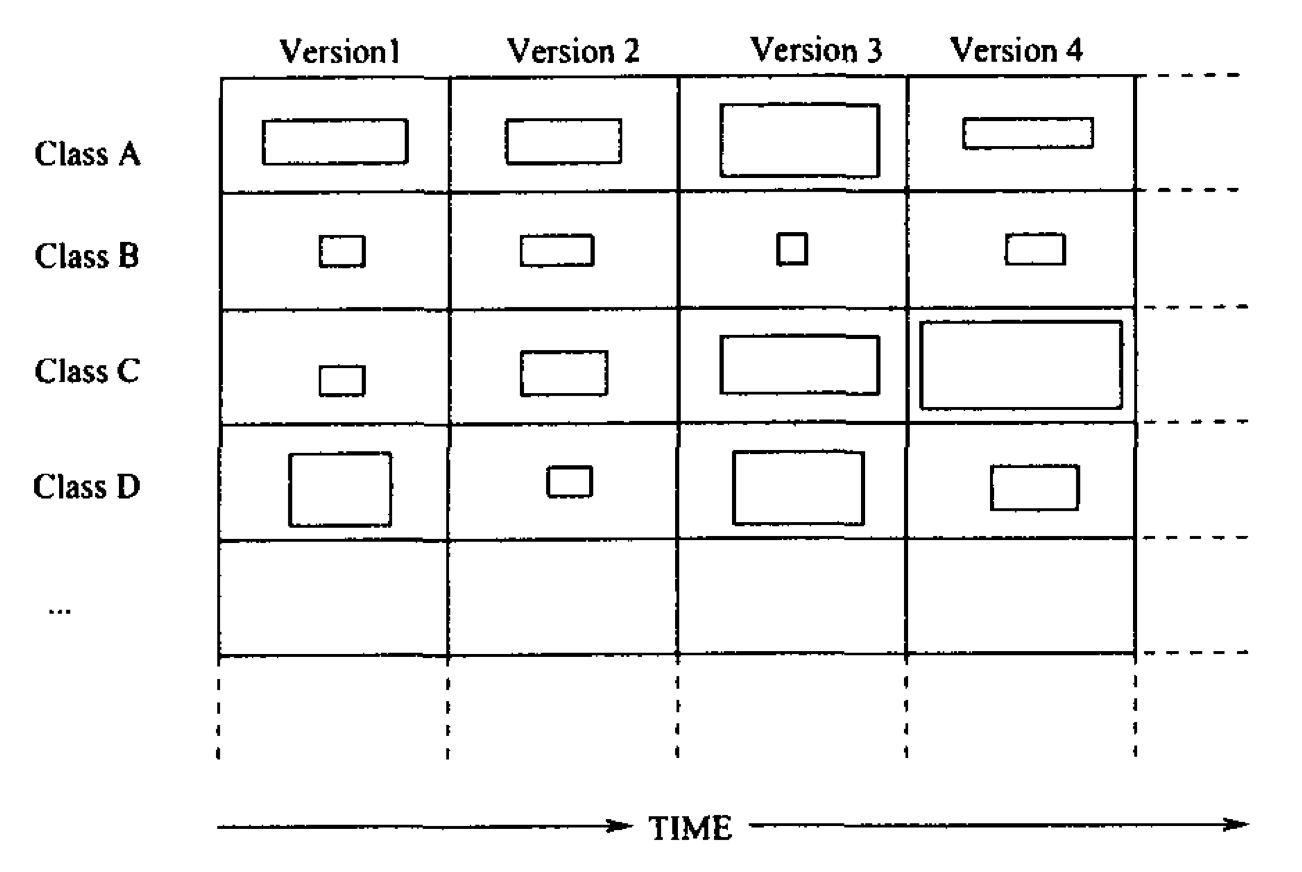
\includegraphics[width=\linewidth]{EvolutionMatrix1.png}
  \caption{A schematic display of the Evolution Matrix}
\endminipage\hfill
\minipage{0.49\textwidth}
  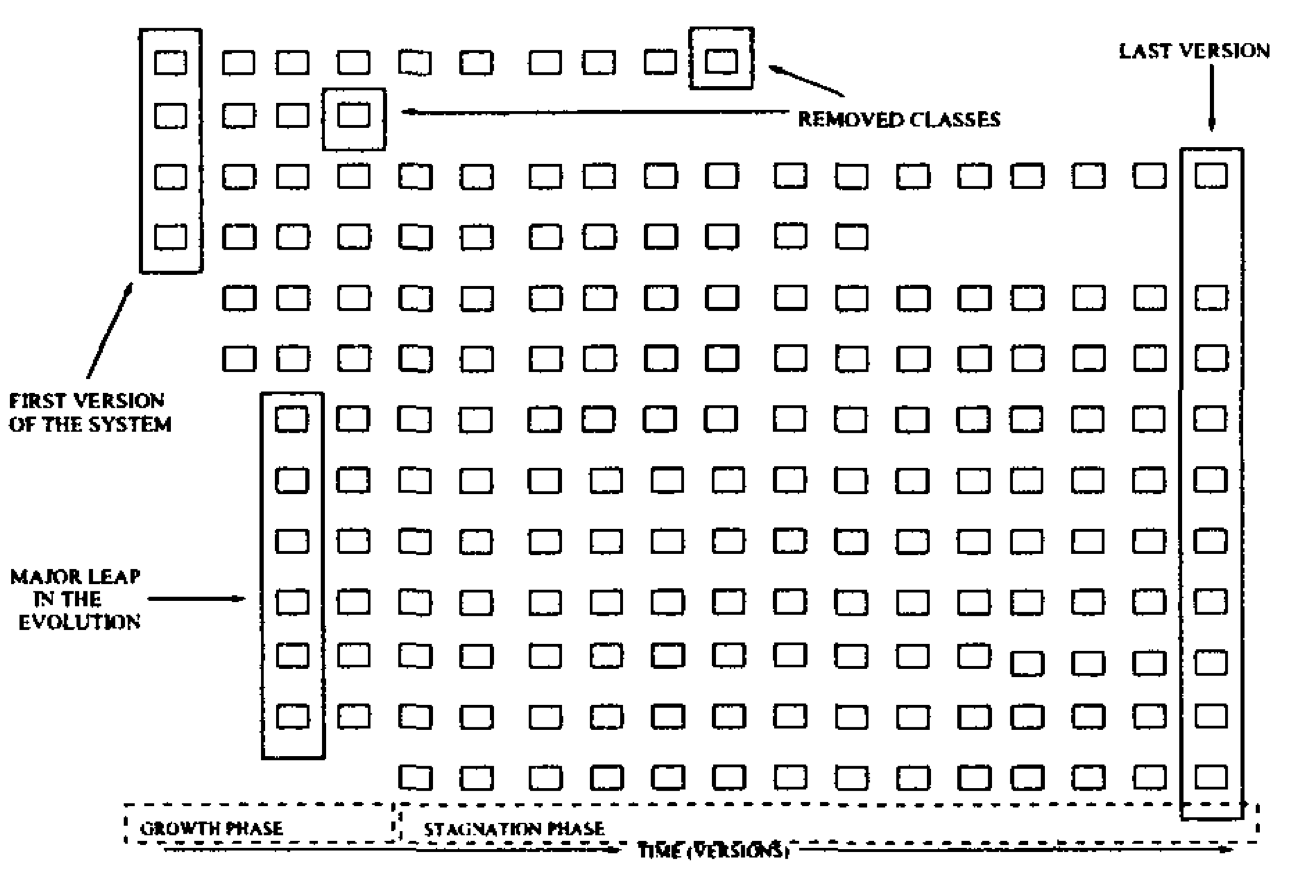
\includegraphics[width=\linewidth]{EvolutionMatrix2.png}
  \caption{Some characteristics of the Evolution Matrix}
\endminipage\hfill
\end{figure}

\newpage

Wettel, in his thesis \cite{Wettel2011}, defined a city metaphor for software visualization that represents software as cities.
 His work represents packages as districts and classes as buildings.
  This metaphor was applied in different contexts related to reverse engineering (program comprehension, software evolution, software quality)
   to demonstrate metaphor's versatility. As a result, he found evidence that his approach works.
    However, he claims that city metaphor brings visual and layout limitations 
    (not all visualization techniques fit well with it). Under those circumstances, he preferred simplicity over the accuracy,
     so he obtained a simple visual language that facilitates comprehension of data. He conducted an experiment of the evidence that the city
      metaphor enables the creation of efficient software visualizations. His approach was implemented by a software visualization tool 
      called CodeCity that supports the city metaphor. 
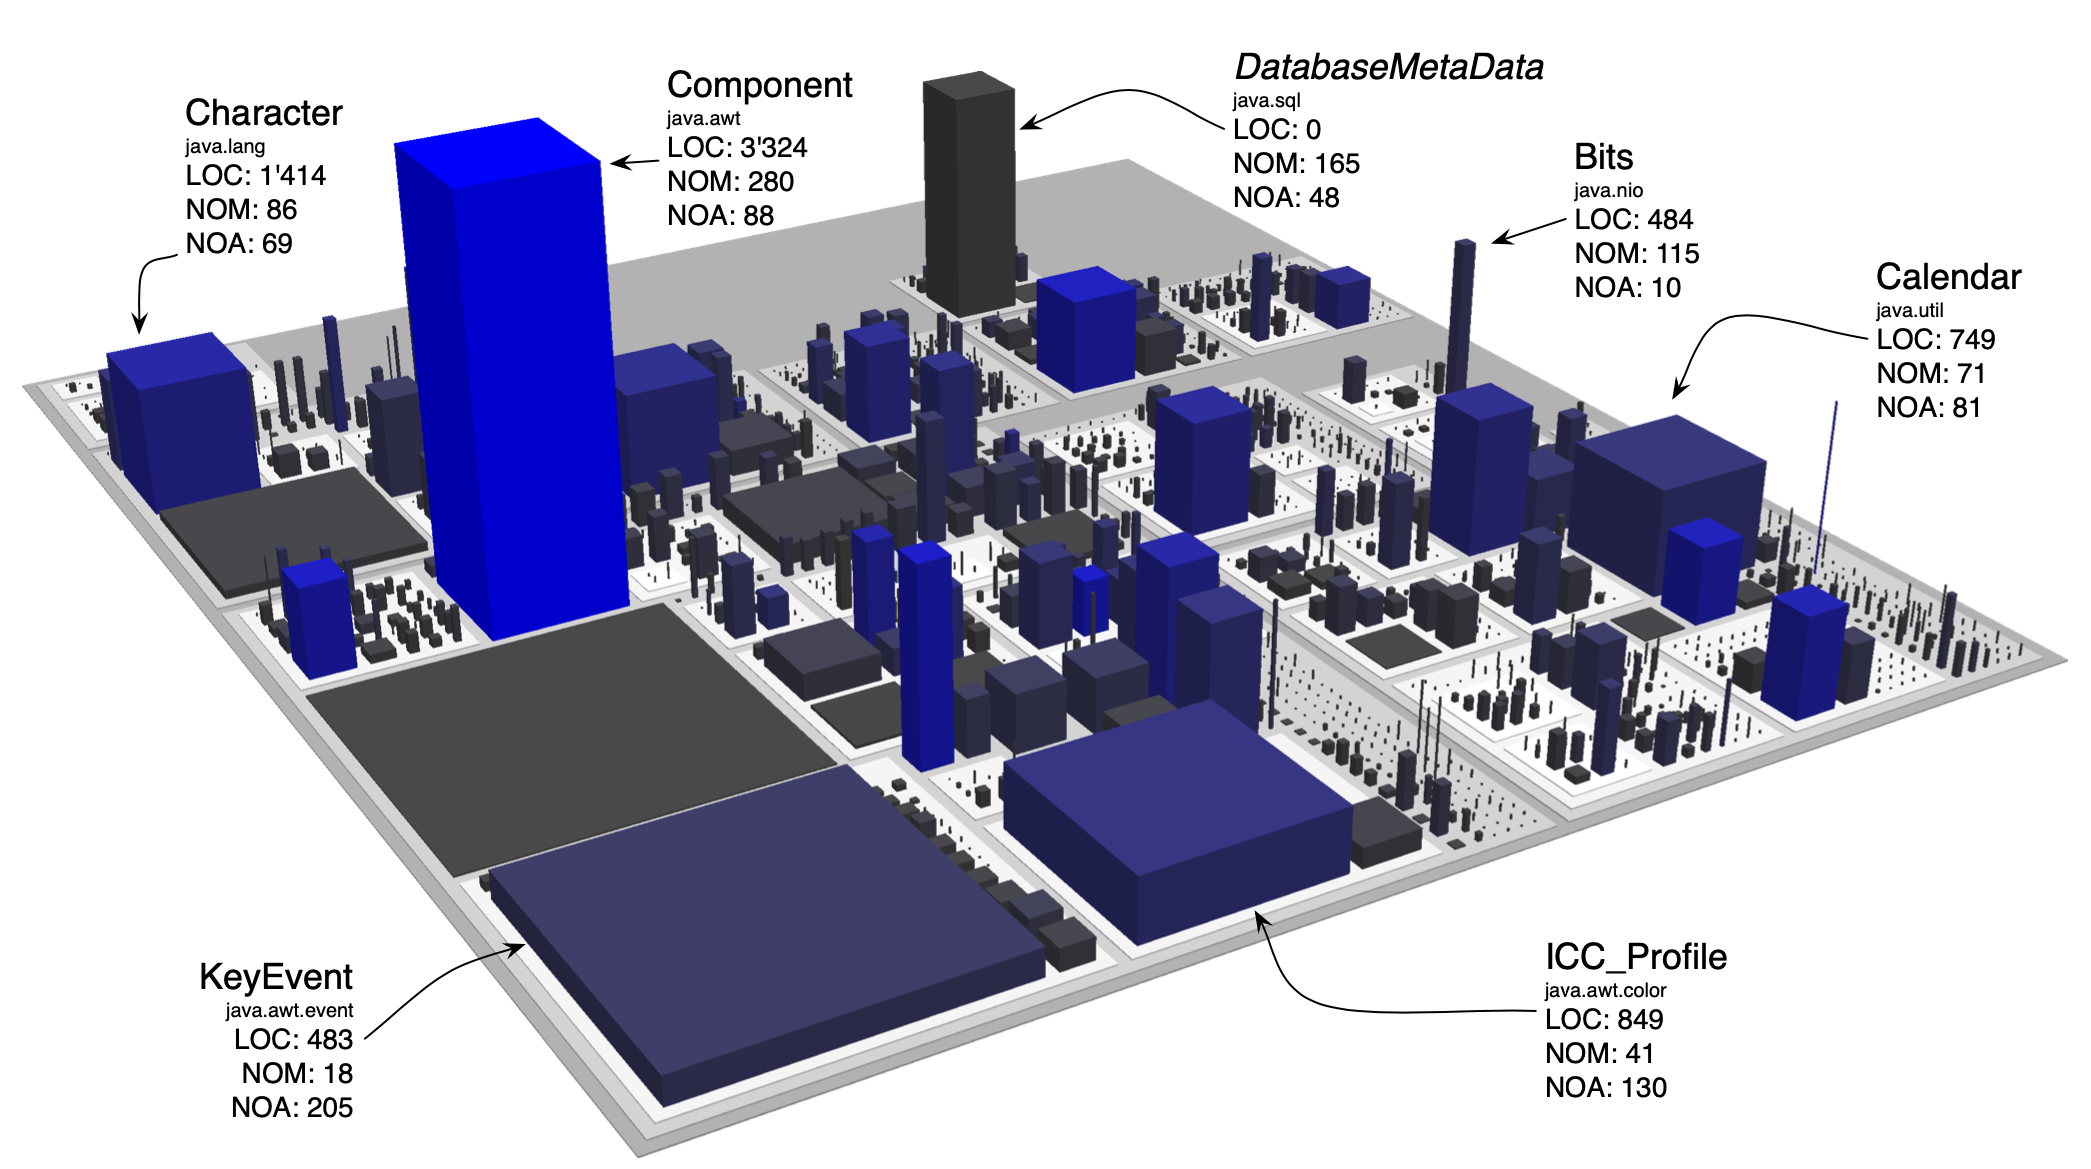
\includegraphics[width=\textwidth]{CodeCity.png}


